\section{\label{sec:internal-experiment}Experiment}

The first experiment is focus on the context switching time.
We implemented a simple application under Contiki.
The application contains two indentical tasks.
The tasks wait for 1ms in the foreground and then goes to the background letting the scheduler runs the next task.
The tasks run in an infinite loop.
The source code of the tasks are shown in the listing \ref{lst:simple-task-code}.

\begin{lstlisting}[style=CStyle, label={lst:simple-task-code}, caption={Source code of the simple task implemented in Contiki}]
PROCESS_THREAD(task, ev, data)
{
    PROCESS_BEGIN();

    while (1)
    {
        PROCESS_PAUSE();
        // Wait for 1ms
        clock_delay_usec(1000);
    }

    PROCESS_END();
}
\end{lstlisting}


We choose to use Contiki for this measurement for its cooperative scheduling.
This kind of scheduling allows us to know when a task is in the foreground and when it goes to the background.
With a preemptive scheduling, in the other hand, we don't know when the task is preempted.
This issue is discussed later in our work.

\subsection{\label{sec:reference-value}Reference value}

We need a reference value for the context switching time in order to develop this benchmarking framework.
This value would allow us to assess the performance of our framework.
Commonly, the context switching time is measured using an oscilloscope.
We updated our simple task by adding GPIO calls in order for the oscilloscope to detect it.
The task will set up a GPIO, wait for 1ms, and then clear the GPIO.
The source code of the updated task is shown in the listing \ref{lst:gpio-task-code}.
The two tasks use different GPIO in order to differenciate them with the oscilloscope.

\begin{lstlisting}[style=CStyle, label={lst:gpio-task-code}, caption={Source code of the task with GPIO calls}]
  PROCESS_THREAD(task, ev, data)
  {
      PROCESS_BEGIN();
  
      while (1)
      {
          PROCESS_PAUSE();
          // Set the GPIO PC3 up
          GPIO_SET_PIN(GPIO_PORT_TO_BASE(GPIO_C_NUM), GPIO_PIN_MASK(3));
          // Wait for 1ms
          clock_delay_usec(1000);
          // Clear the GPIO PC3
          GPIO_CLR_PIN(GPIO_PORT_TO_BASE(GPIO_C_NUM), GPIO_PIN_MASK(3));
      }
  
      PROCESS_END();
  }
\end{lstlisting}

\subsubsection{Measurement setup}

The oscilloscope used for the measurement was the Tektronix MSO 56 available at the Welcome Lab.
We used two channels to measure the voltage of the two GPIOs used by the application.
The measurement is displayed in the figure \ref{fig:measurement-value-wave}.
High value means that the task is running in the foreground.
Low value means that the task is sleeping in the background.

\begin{figure}[!ht]
  \centering
  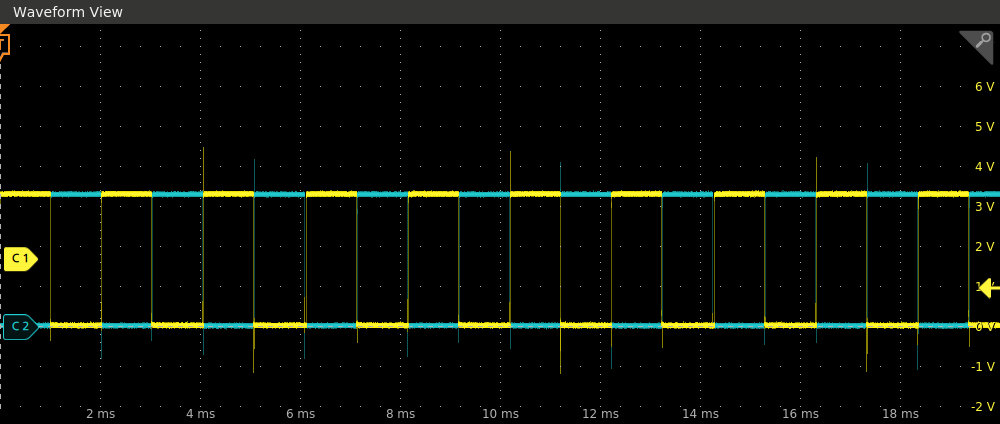
\includegraphics[scale=0.5]{assets/measurement-value-wave.png}
  \caption{\label{fig:measurement-value-wave}Voltage measurement of the two GPIOs; Each color represents a task}
\end{figure}

\subsubsection{Measurement value}

The context switching time is the time during which no task is running.
This is visible with the oscilloscope when both channels are low.

With the oscilloscope, we made four measurements.
The first two measurements are the context switching times from task 1 to task 2 and from task 2 to task 1.
The other two measurements are the time taken by the two tasks.
These last measurements should be arround 1ms.
The measurements are shown in the table \ref{tab:reference-measurement}.

With these results, we can see that the duration of both tasks is 1ms with no variation.
We also extract with this measurement our reference value.
From task 1 to task 2, we have 14.68$\mu$s of context switching time and from task 2 to task 1, we have 14.88$\mu$s.
Our benchmarking framework should compute the context switching time of that same application and output a value between 13.30$\mu$s and 16.26$\mu$s for an error bound of 10\%.

\begin{table}[!ht]
  \centering
  \begin{tabular}{llll}
                        & \multicolumn{3}{c}{Time ($\mu$s)}                              \\ \cline{2-4} 
                        & \multicolumn{1}{c}{Mean} & Min   & \multicolumn{1}{c}{Max} \\ \cline{2-4} 
  From task 1 to task 2 & 14.68                    & 14.35 & 14.79                   \\
  From task 2 to task 1 & 14.88                    & 14.33 & 14.97                   \\
  Duration of task 1    & 1003                     & 1003  & 1003                    \\
  Duration of task 2    & 1003                     & 1003  & 1003                   
  \end{tabular}
  \caption{Context switching times and task durations measured with the oscilloscope Tektronix MSO 56}
  \label{tab:reference-measurement}
\end{table}


\subsection{Methodology}

Before we start to develop our framework, we have contacted and discussed with some of the IoT communities.
Via mailing lists, we communicated with the communities of RIOT OS, Contiki, FreeRTOS, mBed OS and Apache Mynewt.
We also exchanged idea with IoT developers through forums on the web.
Our main concern was to implement a framework that measure the context switching time without altering it.
Unfortunately, the communities and the developpers could not help us.

So we decided two approaches to solve this problem.
The first one is to implement the framework inside the scheduler in the kernel of the RTOS.
The second one is to implement the framework as an external library used by the RTOS that have a minimal impact on the context switching time.

\paragraph{Integration in the kernel}
This approach was abandonned early as the scheduling algorithm is different for each platform.
Some of them are written in assembly language.
We could not implement a generic solution that cover every platform.

\paragraph{Minimal impact framework}
The framework we have developped use the following principle.
Every time a task is executed (inside an infinite loop, from an interrupt, ...) it pings the framework using the \texttt{bench\_ping} call providing its task ID.
By pinging the framework, the task shows that it runs in foreground.
The framework will detect a context switching by comparing the active task ID with the previous one at each ping.
If the ID's do not match, it means that the active task has changed and the framework will compute the elapsed time (computed in ticks) and print it.

\subsubsection{Framework implementation}

The source code of this benchmarking framework is shown in the listing \ref{lst:internal-bench-code}.

\begin{lstlisting}[style=CStyle, label={lst:internal-bench-code}, caption={Source code of the benchmarking framework implemented in Contiki}]
/**
  * Struct that stores benchmarking information.
  * 
  * previous_id: The id of the previous thread that performs a ping;
  * new_id: The id of the current thread that has performed a ping;
  * current_time: the timer
  */
struct BContext {
  uint32_t previous_id;
  uint32_t new_id;
  clock_time_t current_time;
} bench_context;


void bench_ping(uint32_t id) {
  // Save the new id
  bench_context.new_id = id;
  // Save the current time
  // Check for switching context
  if (!check_change()) {
    bench_context.current_time = RTIMER_NOW(); // Ticks
  }
}

int check_change(void) {
  if(bench_context.new_id != bench_context.previous_id) {
    // Compute the difference
    clock_time_t previous = bench_context.current_time;
    clock_time_t current = RTIMER_NOW();
    clock_time_t result = current - previous;

    // Keep the previous id for log
    uint32_t previous_id = bench_context.previous_id;
    // Change previous_id to new_id
    bench_context.previous_id = bench_context.new_id;

    bench_context.current_time = RTIMER_NOW(); // Ticks

    printf("[BENCH_CONTEXT_SWITCHING] %lu %lu %lu\n", previous_id, bench_context.new_id, result);
    
    return 1; // Change occurs
  }
  return 0; // No change
}
\end{lstlisting}


We wanted to make our benchmarking framework hidden for the developer.
But we had no other choice but to create a benchmarking call \texttt{bench\_ping} that the developer need to use in his tasks.
The listing \ref{lst:bench-task-code} shows how we integrate our framework in the simple task.

\begin{lstlisting}[style=CStyle, label={lst:bench-task-code}, caption={Source code of the task with benchmarking framework calls}]
PROCESS_THREAD(task, ev, data)
{
    PROCESS_BEGIN();

    while (1)
    {
        PROCESS_PAUSE();
        bench_ping(TASK_ID);
        // Wait for 1ms
        clock_delay_usec(1000);
    }

    PROCESS_END();
}
\end{lstlisting}

\subsection{\label{sec:internal-setup}Experiment setup}

For this experiment we used the Zolertia RE-MOTE (shown in figure \ref{fig:remote}) with the Contiki RTOS.
This board use a Cortex-M3 at 32 MHz clock speed with 512KB of flash and 32 KB of RAM.
Based on the RFC7228, this board is defined as a class-2 device.

\begin{figure}
  \centering
  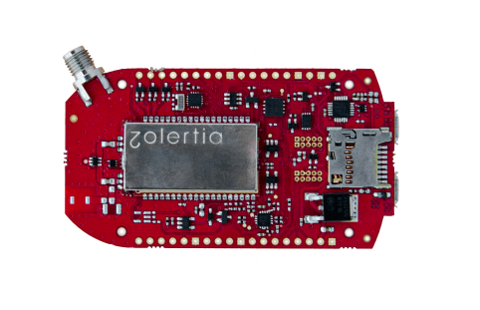
\includegraphics[scale=0.7]{assets/remote.png}
  \caption{\label{fig:remote}Zolertia RE-MOTE board}
\end{figure}

All computation are made in the board so the computer used to retrieve those value is irrelevant.